\section{Peripheral programming}

The camera is composed of 18 pins, where 2 are dedicated to Vdd and Gnd, 2 are part of the serial protocol called \textbf{Serial Camera Control Bus}, 11 are connected to MCU's DCMI peripheral for image acquiring and synchronization, 1 pin is an input for the clock source and the last 2 are for resetting and enabling. Before describing what I did, I would like to spend few words about SCCB and DCMI.
\newline
\newline
Substantially, SCCB is almost identical to I2C. The only difference regards the role of the ACK bit. This protocol doesn't care it, anyway it's generated low as well. However, from the microcontroller side, I enabled another I2C peripheral, another one than whose interfaces with A2D.
\newline
\newline
DCMI is a kind of protocol widespread used in multimedia processing. Although it allows also an higher parallelism, in terms of data bits, the camera chip, provided by OmniVision, has constrained at 8, labeled from $D0$ to $D7$. After having configured, the acquisition of the image works as follows. PXCLK is used as internal synchronizator derived from the XCLK, i.e. the system clock generated by a GPIO of the STMF446. VSYNCH and HREF pins are part of DCMI interface as well. VSYNCH triggers the start and the stop of frame capturing, HREF signal indicates the start/end of a line.

\begin{figure}[H]
\centering
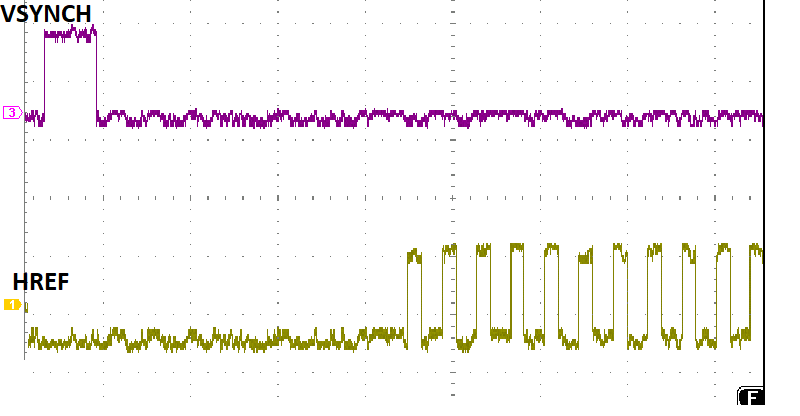
\includegraphics[scale=.9]{Immagini/08}
\label{08}
\caption{Start of frame capturing (top) and sampling line by line (bottom)}
\end{figure}

I guess that another relevant aspect of DCMI is how data are then transferred within microcontroller. This peripheral embeds and works as default by DMA. In fact, when setting DCMI, any option related to DMA's disable cannot be modified. So, in the firmware, I had to declare an array 76800 bytes long, to satisfy image sizing. If I hadn't been constrained by RAM capacity (128Kbyte), I would have used a 153000 long one.
\newline
\newline
I programmed the camera in order to work in single snap shot. The command is user generated on the FPGA side, which sends the command via UART to microcontroller. That UART generates an interrupt when start working; the interrupt launches the start capturing function. When the image transfer has done, I turn the camera off and then I drive the array to the host computer via another UART peripheral of the microcontroller. 
\newline
\newline
The camera embeds a register configuration file of 200 locations around. Not all of them are required to be written to make it work. However I found an example online, where the main ones are highlighted with values to be loaded in them. I modified some of them to make the application compliant with my system. I'm going to list some important configuration settings.

\begin{table}[H]
\centering
\begin{tabular}{p{0.5\textwidth}p{0.4\textwidth}}

\textbf{Bit(s) name}&\textbf{Description}\\ \hline
(COM7) Color Bar & Enable\\
(COM7) Output format & RGB and QVGA\\
(MVFP) Mirror	& Normal Image Acquisition (No mirroring)\\
(CLKRC) Clock prescaler & Prescaler disabled for PXCLK\\
(COM16) Threshold and de-noise auto adjustment & Both enabled\\
\hline
\end{tabular}
\caption{Camera configuration}
\end{table}

\begin{figure}[H]
\centering
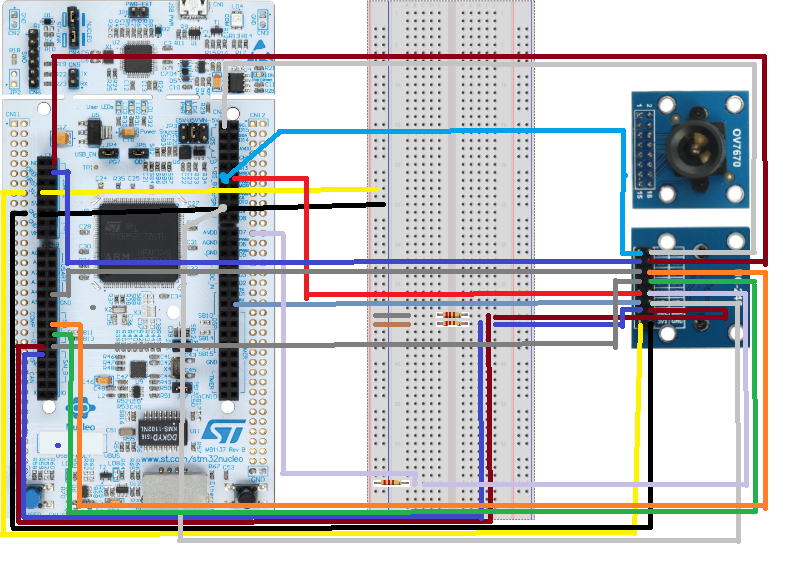
\includegraphics[scale=.9]{Immagini/10}
\label{10}
\caption{Connection between MCU and camera}
\end{figure}

\begin{figure}[H]
\centering
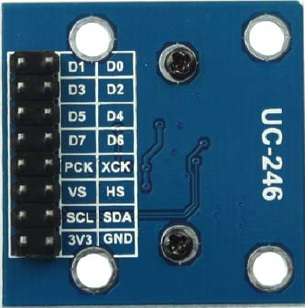
\includegraphics{Immagini/11}
\label{11}
\caption{Camera's bottom side}
\end{figure}

\begin{table}[H]
\centering
\begin{tabular}{p{0.2\textwidth}p{0.4\textwidth}p{0.2\textwidth}}

\textbf{GPIO}&\textbf{Morpho Connector}&\textbf{Description}\\ \hline
PF0 & D68 & I2C2\_SDA\\ 
PF1 & D69 & I2C2\_SCK\\ 
PA8 &     & RCC\_MCO1 (25 Mhz) -> XCLK\\
PA4 & D24 & DCMI\_HSYNC\\
PG9 & D0  & DCMI\_VSYNC\\
PA6 & D12 & DCMI\_PXCLK\\
PC6 & D16 & DCMI\_D0\\
PC7 & D21 & DCMI\_D1\\
PC8 & D43 & DCMI\_D2\\
PC9 & D44 & DCMI\_D3\\
PE4 & D57 & DCMI\_D4\\
PD3 & D55 & DCMI\_D5\\
PE5 & D58 & DCMI\_D6\\
PE6 & D59 & DCMI\_D7\\
\hline
\end{tabular}
\caption{Camera: GPIOs involved}
\end{table}